\documentclass[sigconf]{acmart}
\usepackage{amsmath}
\usepackage{graphicx}
\usepackage{caption}
\usepackage{subcaption}
\usepackage{algorithm}
\usepackage{algpseudocode}

\newcommand{\vect}[1]{\boldsymbol{#1}}


\AtBeginDocument{%
  \providecommand\BibTeX{{%
    \normalfont B\kern-0.5em{\scshape i\kern-0.25em b}\kern-0.8em\TeX}}}

\setcopyright{acmcopyright}
\copyrightyear{2021}
\acmYear{2021}
\acmDOI{0.0/0.0}

\begin{document}

%%
%% The "title" command has an optional parameter,
%% allowing the author to define a "short title" to be used in page headers.
\title{Technical Breakdown of Position Based Fluid}

%%
%% The "author" command and its associated commands are used to define
%% the authors and their affiliations.
%% Of note is the shared affiliation of the first two authors, and the
%% "authornote" and "authornotemark" commands
%% used to denote shared contribution to the research.
\author{Qingyuan Qie}
\email{will.qie@mail.utoronto.ca}
\affiliation{%
  \institution{University of Toronto}
  \city{Toronto}
  \state{ON}
  \country{Canada}
}

\author{Changlin Su}
\email{sheldon.su@mail.utoronto.ca}
\affiliation{%
  \institution{University of Toronto}
  \city{Toronto}
  \state{ON}
  \country{Canada}
}

%%
%% By default, the full list of authors will be used in the page
%% headers. Often, this list is too long, and will overlap
%% other information printed in the page headers. This command allows
%% the author to define a more concise list
%% of authors' names for this purpose.
\renewcommand{\shortauthors}{Changlin and Qingyuan}

%%
%% The abstract is a short summary of the work to be presented in the
%% article.
\begin{abstract}
  This paper provides a technical breakdown of implementing a parallel version of the Position Based Fluids(PBF) method. We discussed the simulation algorithms of PBF, the effects of different confinements in the algorithms. We also go in depth of the data structures used to implement the algorithms efficiently. Due to the highly parallelizable nature of the algorithm, we provided a implementation using the CUDA platform which achieves realtime simulation with a particle count of 12k. A CPU version is also available.
\end{abstract}

%%
%% The code below is generated by the tool at http://dl.acm.org/ccs.cfm.
%% Please copy and paste the code instead of the example below.
%%
\begin{CCSXML}
  <ccs2012>
     <concept>
         <concept_id>10010147.10010371.10010352.10010379</concept_id>
         <concept_desc>Computing methodologies~Physical simulation</concept_desc>
         <concept_significance>500</concept_significance>
         </concept>
   </ccs2012>
\end{CCSXML}
  
\ccsdesc[500]{Computing methodologies~Physical simulation}

%%
%% Keywords. The author(s) should pick words that accurately describe
%% the work being presented. Separate the keywords with commas.
\keywords{Fluids Simulation, Physics-Based Animation}

%%
%% This command processes the author and affiliation and title
%% information and builds the first part of the formatted document.
\maketitle

\section{Introduction}
In Position Based Fluids(PBF) method, fluids are simulated with discrete particles, the surfaces of the fluids are reconstructed at render time based on the position of the underlying particles. In each time step, the PBF method first predicts the positions and velocity. Then it corrects the particle positions by enforcing the incompressibility constraints. The new velocity of the particles are computed from the new positions and the original positions of the particles.

Algorithm \ref{alg:simulation_step} is an overview of a simulation step in PBF method.

\begin{algorithm}
  \caption{simulation step}
  \label{alg:simulation_step}
  \begin{algorithmic}[1]
    \For{all particles $i$}: \Comment{Fluid advect}
    \State apply forces $\vect{v}_i = \vect{v}_i + \Delta t f_{ext}$
    \State predict position $\vect{x}_i^* = \vect{x}_i + \Delta t \vect{v_i}$
    \EndFor
    \For{all particles $i$}:
    \State find neighboring particles $F(\vect{x}_i^*)$
    \EndFor
    \While{$iter < solverIterations$}: \Comment{Iterativly solves imcompressibility constraints}
      \For{all particles $i$}:
      \State calculate $\lambda_i$
      \EndFor
      \For{all particles $i$}:
      \State calculate $\Delta \vect{p}_i$
      \State perform collision detection and response
      \EndFor
      \For{all particles $i$}:
      \State update position $\vect{x}_i^* = \vect{x}_i^* + \Delta \vect{p}_i$
      \EndFor
    \EndWhile
    \For{all particles $i$}:
    \State update velocity $\vect{v}_i = \frac{1}{\Delta t}(\vect{x}_i^*-\vect{x}_i)$
    \State apply viscosity
    \State update position $\vect{x}_i = \vect{x}_i^*$
      \EndFor
  \end{algorithmic}
\end{algorithm}

\section{Enforcing incompressibility}
For particle $i$ at position $p_i$, we compute the density of the fluid around particle $i$ using the estimator:
\begin{equation}
  \rho_{F(i)} = \sum_{j \in F(i)} m_j W_{poly6}(\vect{p}_i - \vect{p}_j, h)
\end{equation}
where $\rho_0$ is the rest density of the fluid, $m_j$ is the mass of the particle $j$, $h$ is a constant, and $W$ is the Poly6 kernel from [TODO: insert citation]. $F$ is the neighbor function that returns the neighboring particle of particle $i$.

The Poly6 kernel is defined as follows,
\begin{equation*}
  W_{poly6}(\vect{r}, h) = \frac{315}{64 \pi h^9}
  \begin{cases}
    (h^2 - r^2)^3 &\text{0 $\leq r \leq h$} \\
    0 &\text{otherwise}
  \end{cases}
\end{equation*}
where $r$ is the norm of $\vect{r}$. Combine equation (1) and the definition of poly6, we can notice that if the distance between particle $i$ and $j$ is greater than $h$, particle $j$ does not contribute to the density around particle $i$. Thus the neighbor-finding algorithm and need to find the particles whose distance to particle $j$ is smaller or equal to $h$, we will discuss the detail of the neighbor-finding algorithm later.

Then we introduce the constant density constraints $C_i$. For particle $i$, we have,
\begin{equation}
  C_i(\vect{p}) = \frac{\rho_i}{\rho_0} - 1
\end{equation}
where $\rho_0$ is a constant that denotes the rest density of the fluid, and $\vect{p}$ is the position of all the particles in the system.

Since we want the density around each particle is always equal to $\rho0$, we want to find a particle correction $\Delta(\vect{p})$ such that,
\begin{equation}
  C(\vect{p} + \vect{\Delta(\vect{p})}) = 0
\end{equation}

The solution to (3) is found by a series of Newton steps along the constraint gradient,
\begin{equation}
  \Delta(\vect{p}) \approx \nabla C(\vect{p})\lambda
\end{equation}
\begin{align*}
  C(\vect{p} + \vect{\Delta(\vect{p})}) &\approx C(\vect{p}) + \nabla C^T \Delta \vect{p} = 0 \tag*{(5)}\\
  &\approx C(p) + \nabla C^T \nabla C \lambda = 0 \tag*{(6)}
\end{align*}
And the gradient of the constraint $C_i$ with respect to a particle $k$ is given by,
\begin{equation}
  \nabla_{\vect{p}_k}C_i = \frac{1}{\rho_0}\sum_{j} \nabla_{\vect{k}}W(\vect{p}_i-\vect{p}_j, h) \tag*{(7)}
\end{equation}
Which has two different cases based on whether $k$ is a neighboring particle or $k$ is the particle $i$ itself,
\begin{equation*}
  \nabla_{\vect{p}_k}C_i = \frac{1}{\rho_0} 
  \begin{cases}
    \sum_{j} \nabla_{\vect{p}_k}W(\vect{p}_i-\vect{p}_j, h) &\text{if $k=i$}\\
    - \nabla_{\vect{p}_k}W(\vect{p}_i-\vect{p}_j, h) &\text{otherwise}
  \end{cases}
  \tag*{(8)}
\end{equation*}
The original paper uses the Spiky kernel fot the gradient computation, which is defined as,
\begin{equation*}
  \nabla W_{spiky}(\vect{r}, h) = -\frac{45}{64 \pi h^6}
  \begin{cases}
    (h - r)^2 \hat{\vect{r}} &\text{0 $\leq r \leq h$} \\
    0 &\text{otherwise}
  \end{cases}
\end{equation*}
where $\hat{r}$ is the normalized $\vect{r}$.

Plug (8) into (6) and solves for $\lambda$ yields,
\begin{equation}
  \lambda_i = -\frac{C_i(\vect{p})}{\sum_k |\nabla_{\vect{p}_k} C_i|^2} \tag*{(9)}
\end{equation}
Then the position correction $\Delta \vect{p}_i$ including affect from neighboring particles is
\begin{equation}
  \Delta \vect{p}_i = \frac{1}{\rho_0} \sum_j (\lambda_i + \lambda_j) \nabla W(\vect{p}_i - \vect{p}_j , h) \tag*{(12)}
\end{equation}
And we have the position update formula,
\begin{equation}
  \vect{p}_i^* = \vect{p}_i + \Delta \vect{p}_i \tag*{(13)}
\end{equation}

\section{Tensile Instability}
The original PBF paper adds an artificial pressure to mitigate the issue of particle clamping. It introduced an additional correction coefficient defined as,
\begin{equation}
  s_{corr} = - k \left(\frac{W(\vect{p}_i-\vect{p}_j, h)}{W(\Delta \vect{q}, h)} \right)^n \tag*{(14)}
\end{equation}
where $\Delta \vect{q}$ is a point some fixed distance inside the smoothing kernel radius and $k$ is a small positive constant. In our implementation, we take $k=0.1, |\Delta \vect{q}| = 0.1h$ and $n=4$. Then the modified position update formula becomes,
\begin{equation}
  \Delta \vect{p}_i = \frac{1}{\rho_0} \sum_j (\lambda_i + \lambda_j + s_{corr}) \nabla W(\vect{p}_i - \vect{p}_j , h) \tag*{(15)}
\end{equation}

\section{Vorticity Confinement and Viscosity}
The original PBF paper implemented vorticity to replace lost energy. However, due to the time constraint, we did not implement vorticity confinement.

We implemented viscosity, which is defined as follows,
\begin{equation}
  \vect{v}_i^* = \vect{v}_i + c \sum_j \vect{v}_{ij} \cdot W(\vect{p}_i-\vect{p}_j, h) \tag*{16}.
\end{equation}
where $\vect{v}_{ij} = \vect{v}_j - \vect{v}_i$. The parameter $c$ is chosen to be 0.001 in our simulation after a few trail and error.
The viscosity is important for convincing fluid motion. Figure \ref{fig:viscosity} shows the effect of the viscosity. When viscosity is not implemented, the particles are more scattered and have the tendency of not moving together, which is not realistic. With viscosity implemented, the fluid is more ``thick" visually and thus more similar to how real water moves.
\begin{figure}
  \centering
  \begin{subfigure}{.5\textwidth}
    \centering
    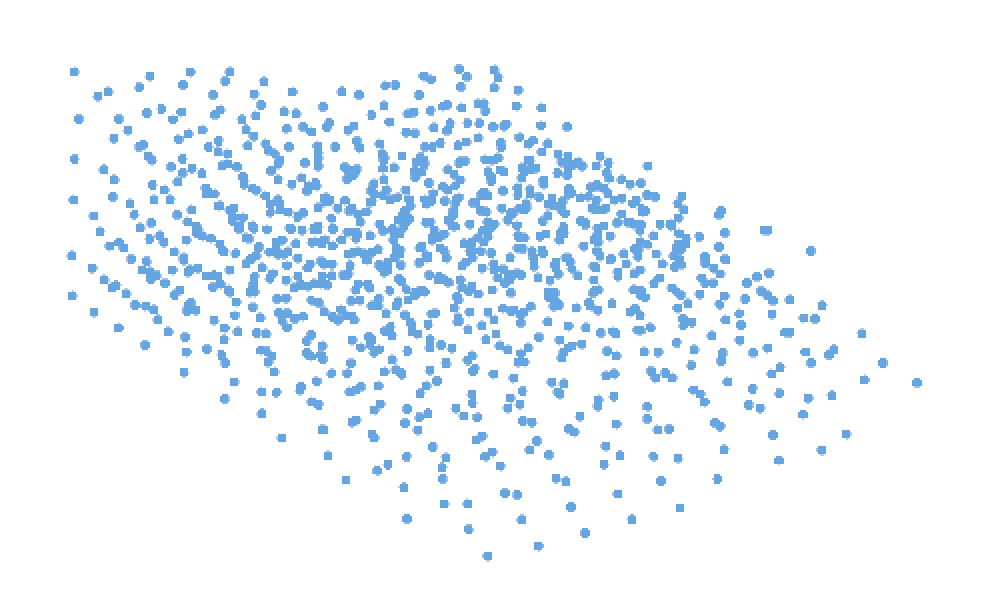
\includegraphics[width=.6\linewidth]{image/with-viscosity.png}
    \caption{With Viscosity Implemented}
    \label{fig:with-viscosity}
  \end{subfigure}
  \begin{subfigure}{.5\textwidth}
    \centering
    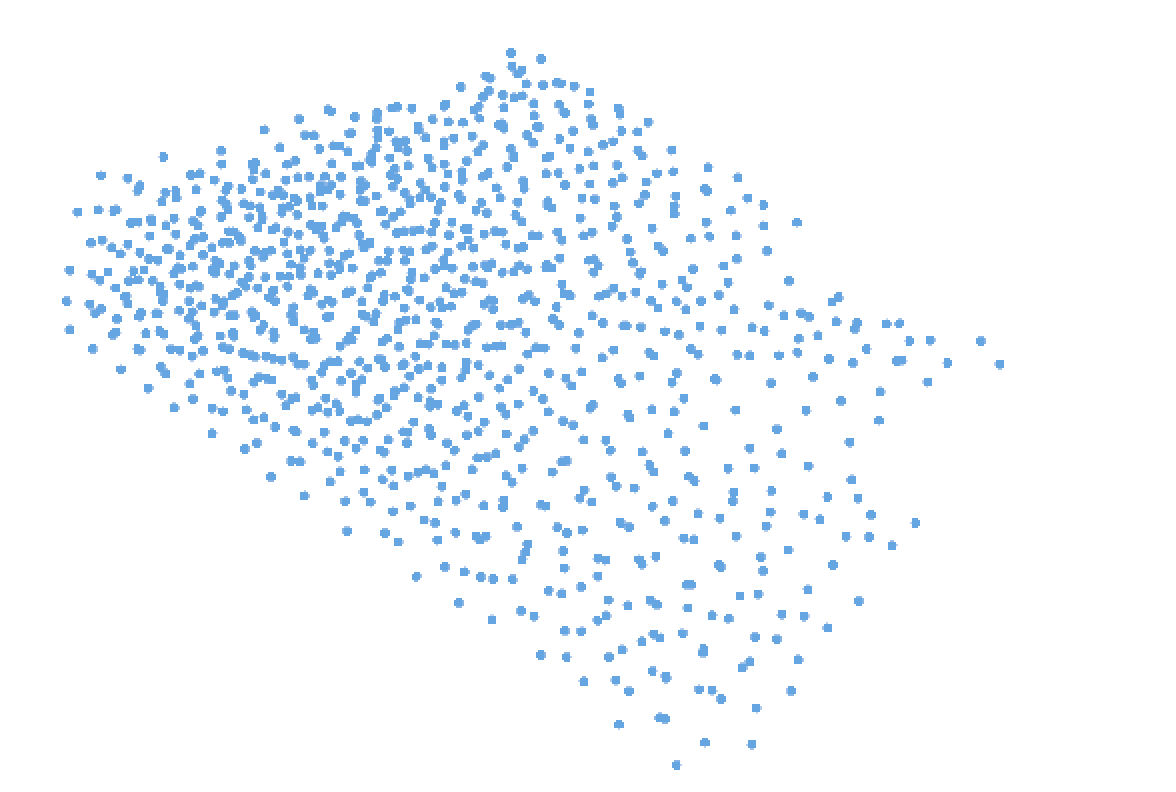
\includegraphics[width=.6\linewidth]{image/without-viscosity.png}
    \caption{Without Viscosity Implemented}
    \label{fig:without-viscosity}
  \end{subfigure}
  \caption{Comparison of the fluid motion with/without viscosity implemented, taken at the same time step.}
\label{fig:viscosity}
\end{figure}

\section{Boundary and Collision Response}
In our implementation, the fluid is confined in a cuboid whose surfaces are parallel to the coordinate planes. We deploy a simple collision scheme as describe in [TODO: CITATION]. Particles that goes out of bound in the fluid advect is clamped into the cuboid with an small distance to the boundary, and velocity of the particle is set to 0.

\section{Grid-based neighbor finding}
The Poly6 and Spiky function both return 0 when the distance of two particles is greater than $h$. Therefore, we adapted the grid-based neighbor finding algorithm described in [TODO: CITATION]. We implemented the CPU version ourselves, and we modified the source code of [TODO: CITATION] for CUDA version. 

\section{Implementation details}
Table \ref{table:name_map} shows the correspondence of algorithm steps to the name of the functions in our code. Since Algorithm \ref{alg:simulation_step} is highly parallelizable with the update of each particle can be computed in parallel, we launch one thread for each particle in the CUDA implementation.

\begin{center}
  \begin{tabular}{| c | c |}
    \hline
    Line Number & CUDA Kernel Name\/ CPU Function Name  \\
    \hline
    1 - 4, 14 & advect \\
    \hline
    5 - 7 & build\_grid \\
    \hline
    9 - 11 & compute\_lambda \\
    \hline
    12-15 & compute\_delta\_position \\
    \hline
    16-19 & update\_position \\
    \hline
    21 & update\_velocity \\
    \hline
    22 & viscosity\_confinement \\
    \hline
  \end{tabular}
  \captionof{table}{Actual Function name to the pseudo-code in Algorithm \ref{alg:simulation_step} \label{table:name_map}}
\end{center}


\end{document}
\endinput